\section{Results}

\subsection{Sequence of MTF-1 is conserved in different organisms.}

We fetched the MTF-1 gene of different eukaryotic organisms from NCBI protein database, and did a multiple sequence alignment. The organisms used in MSA and the accession number is listed in supplementary material.


The MSA showed that peptide sequence of MTF-1 is conserved in different eukaryotic organisms, as is shown in the figure below. We also built a phylogenetic tree using the MSA data as is shown in the figure below.

\begin{figure}[H]
    \centering
    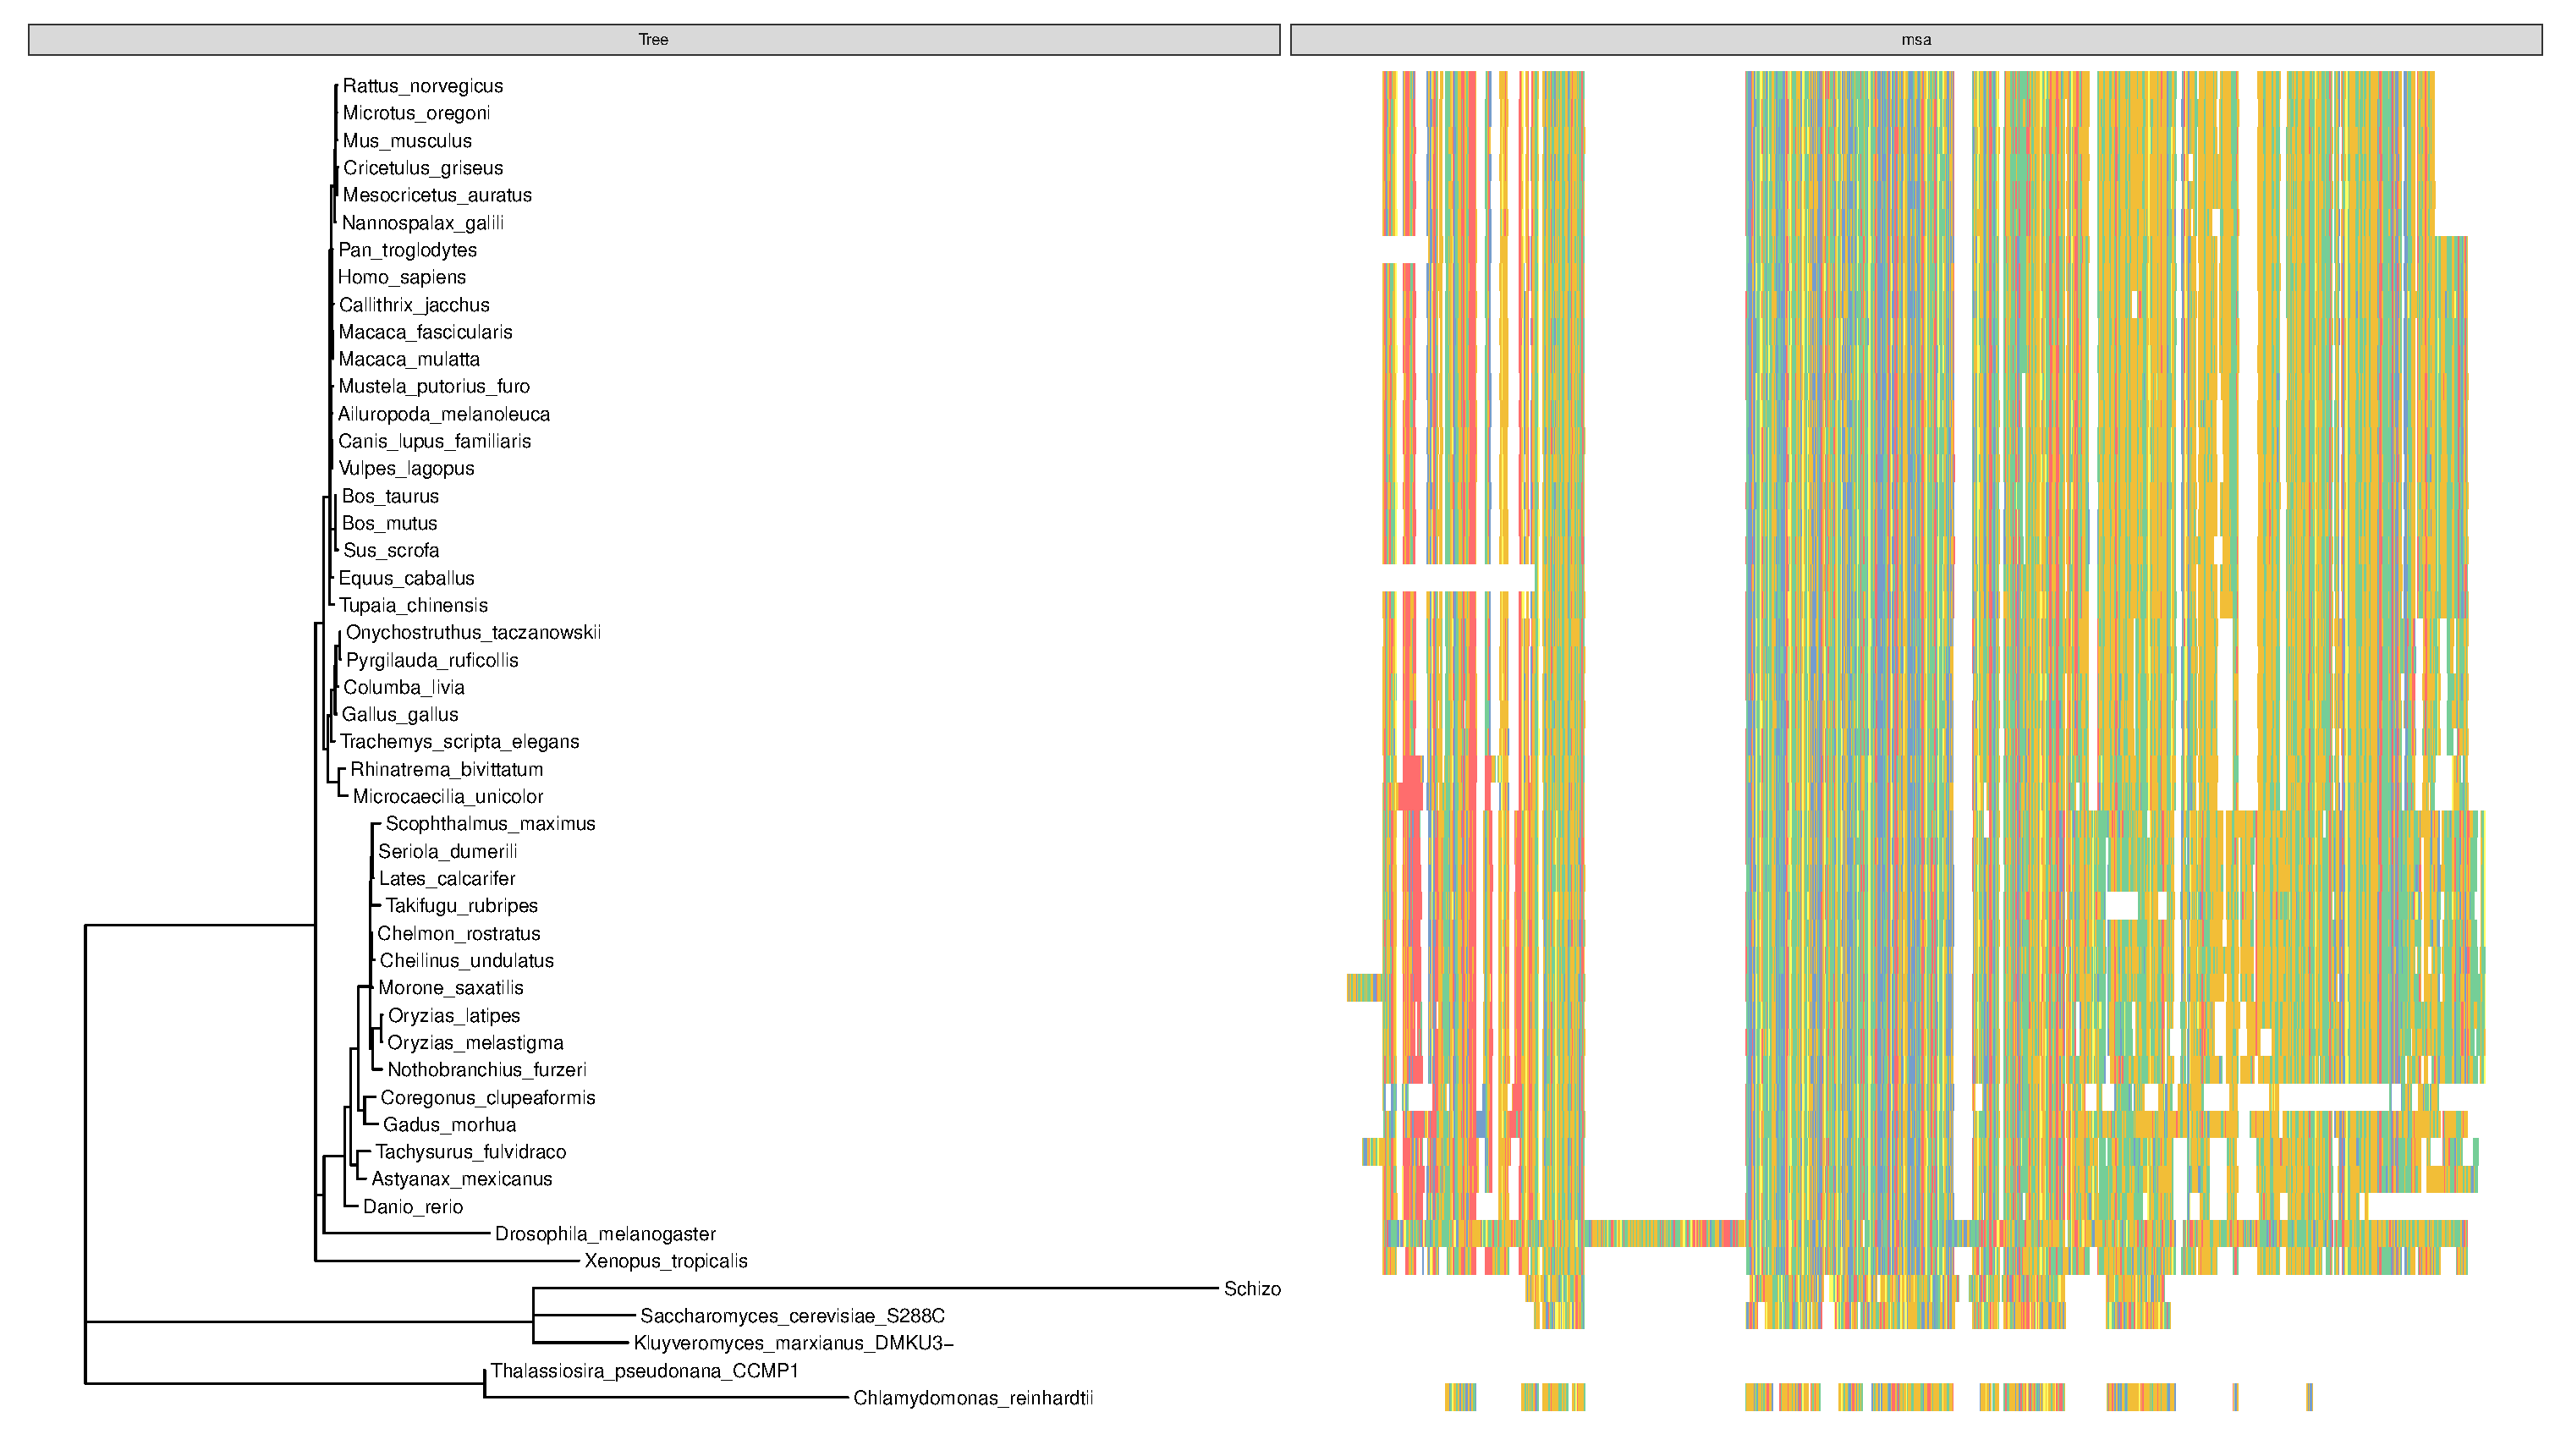
\includegraphics[width=1\textwidth]{image/MSAT.eps}
    \caption{MSA Results (right) and Phylogenetic tree (left) of MTF-1}
    \label{MSAT}
\end{figure}

From the figure, we can find that, in spite of few sequences, MTF-1 in most of the selected organism share similar peptide sequence patterns, which indicates that MTF-1 is conserved in the evolution.

As can be seen in the phylogenetic tree, \textit{Pan troglodytes} or the common chimpanzee shares the closest ancestor with humans. While the fruit fly, \textit{Drosophila melanogaster}, has distinctive MTF-1 sequence with a ~150bp insertion. These results is reasonable and consistent with previous results.

Then we analysed the nucleotide sequence of MTF-1 in the genome of different organisms, and we found that in most organisms, like \textit{Homo sapiens} and \textit{Mus musculus}, there are 7-9 exons in the MTF-1 gene, and they are spliced in a similar way. The related results of human MTF-1 is shown in the figure below.

\begin{figure}[H]
    \centering
    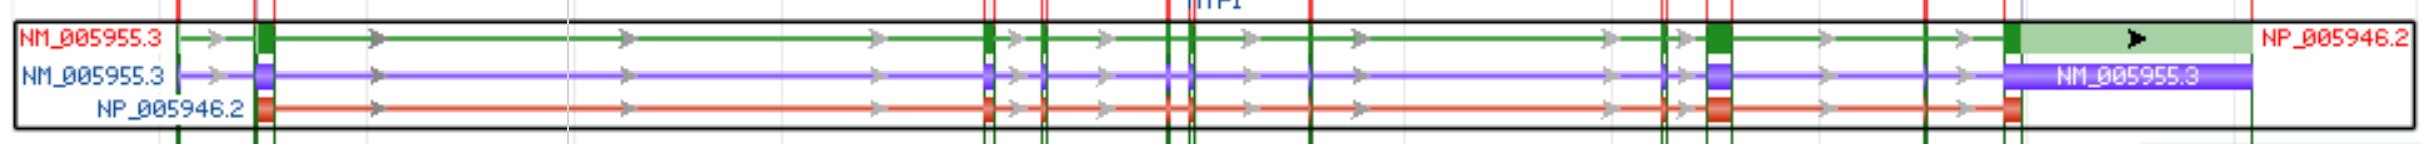
\includegraphics[width=1\textwidth]{image/MTFE.png}
    \caption{Human MTF-1 exons}
    \label{MSAT}
\end{figure}

\subsection{MTF-1 may be an unstable hydrophilic protein.}

Using Expasy ProtParam\upcite{gasteiger2005protein} to analysis mammalian MTF-1 sequences, we found that most of the MTF-1 are hydrophilic, with the average GRAVY\upcite{kyte1982simple} around -0.5. Moreover, Estimated half-life of MTF-1 in many organisms are about 30 hours, which indicates that the protein is unstable.

\begin{figure}[H]
    \centering
    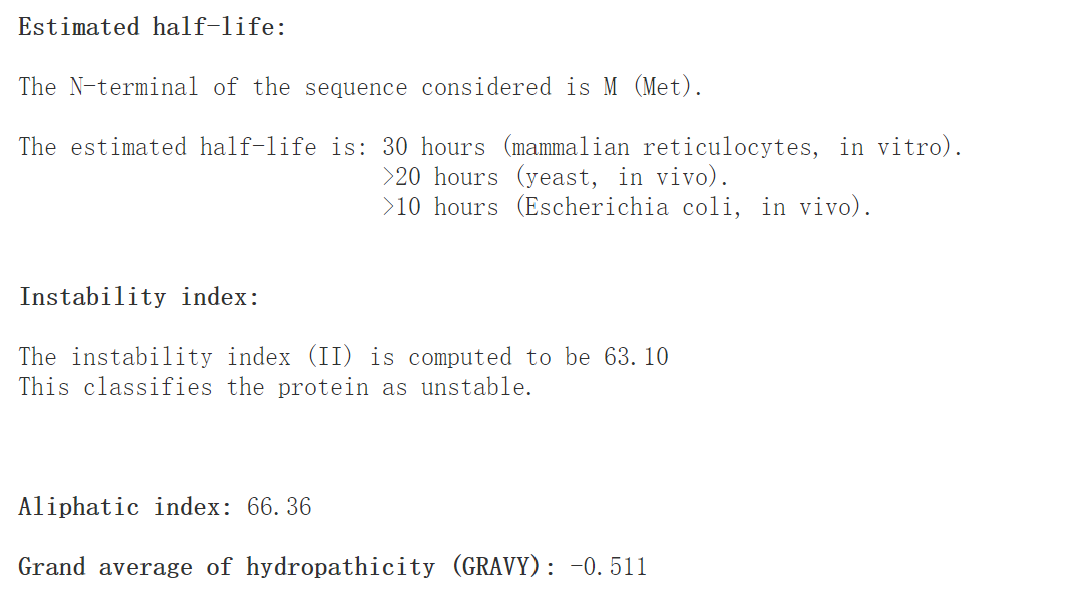
\includegraphics[width=0.7\textwidth]{image/EXPP.png}
    \caption{Part of Human MTF-1 Expasy ProtParam results}
    \label{EXPP}
\end{figure}

Detailed protparam report of human MTF-1 is shown in Supplementary material.

We also performed a TMPred analysis on human MTF-1 to find the hydrophobic region, and the output figure is shown below.

\begin{figure}[H]
    \centering
    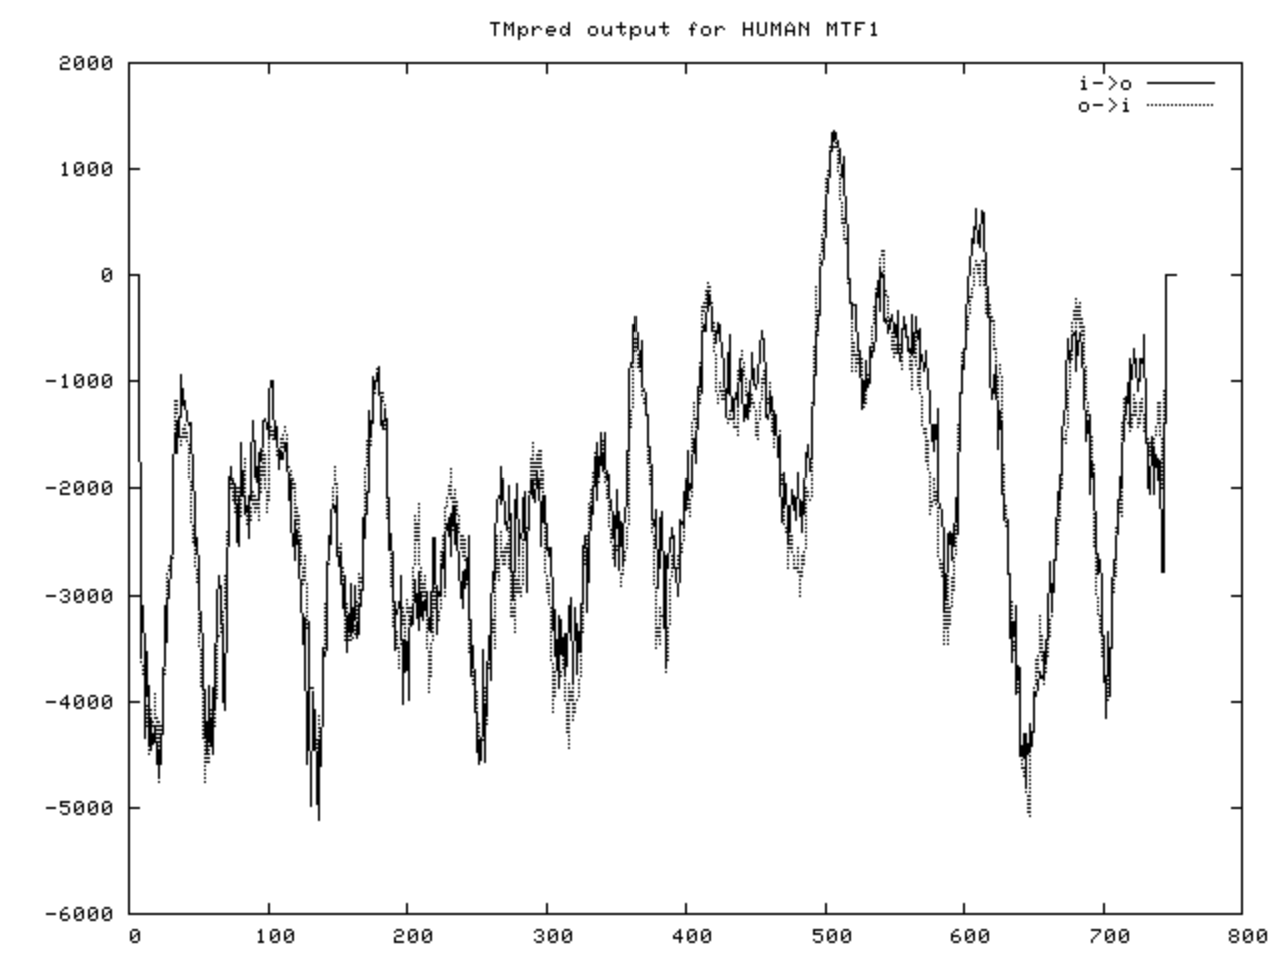
\includegraphics[width=0.7\textwidth]{image/TMPRED.png}
    \caption{Part of Human MTF-1 Expasy TMPred results}
    \label{TMPRED}
\end{figure}

Since MTF-1 is not a membrane protein, it is reasonable that no significant hydrophobic region is found.

\subsection{MTF-1 has nuclear localization signal and zinc finger domains which help it to bind metal response elements.}

Since sequence of MTF-1 is conserved in different eukaryotic organisms, we wanted to find out if there is certain motifs or domains in the MTF-1 conserved region. The sequence used in this subsection is human MTF-1.

Nuclear localization signal is found using cNLS Mapper\upcite{kosugi2009systematic}, with a cut off set to 2.0. The NLS is PETKRKEVKR, which is consistent to the manually annotated KRKEVK signal. The results given by cNLS Mapper is shown below.

\begin{figure}[H]
    \centering
    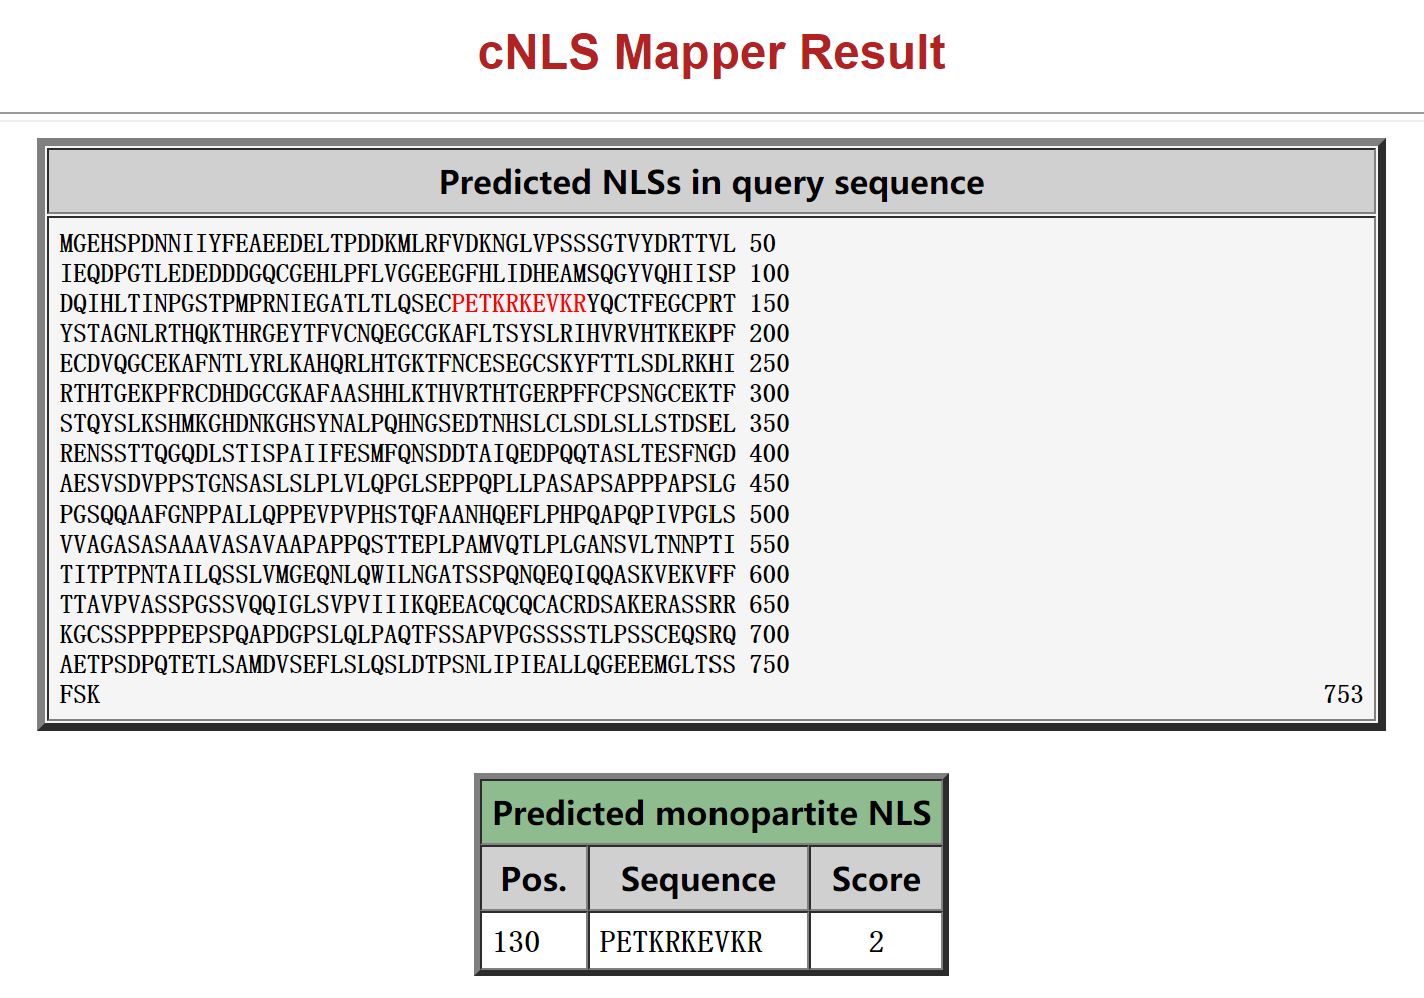
\includegraphics[width=0.7\textwidth]{image/NLSP.png}
    \caption{cNLS Mapper Results (Human MTF-1)}
    \label{NLSP}
\end{figure}

A common domain in transcription factors is the zinc finger domain, and we found 6 ZF domains in human MTF-1 protein using Interactive PWM predictor\upcite{persikov2014novo}, as is shown in the figure below.

\begin{figure}[H]
    \centering
    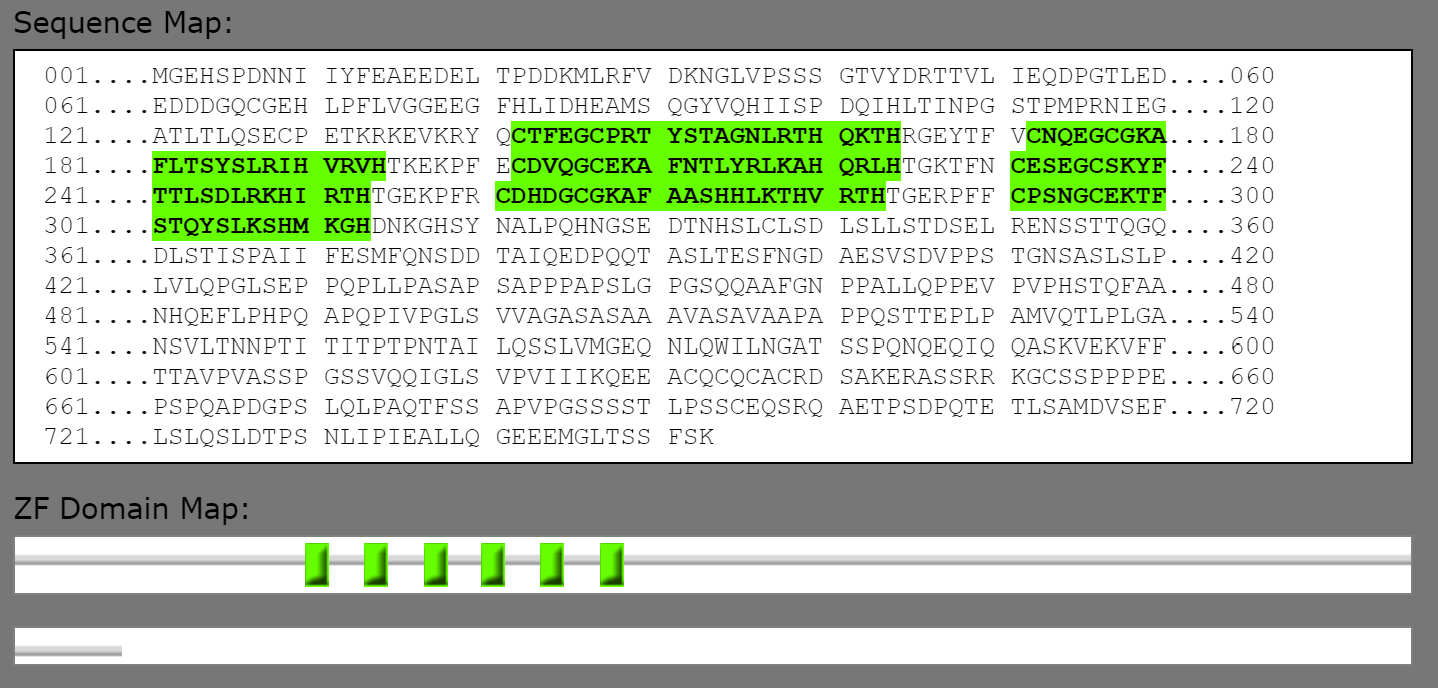
\includegraphics[width=0.7\textwidth]{image/ZFO.png}
    \caption{cNLS Mapper Results (Human MTF-1)}
    \label{HZFP}
\end{figure}

For those MTF-1 in other organisms, the similar zinc finger domain pattern can be found. Here we show \textit{Mus musculus} and \textit{Drosophila melanogaster} as examples.
\begin{figure}[H]
    \centering
    \subfigure[Mouse MTF-1] {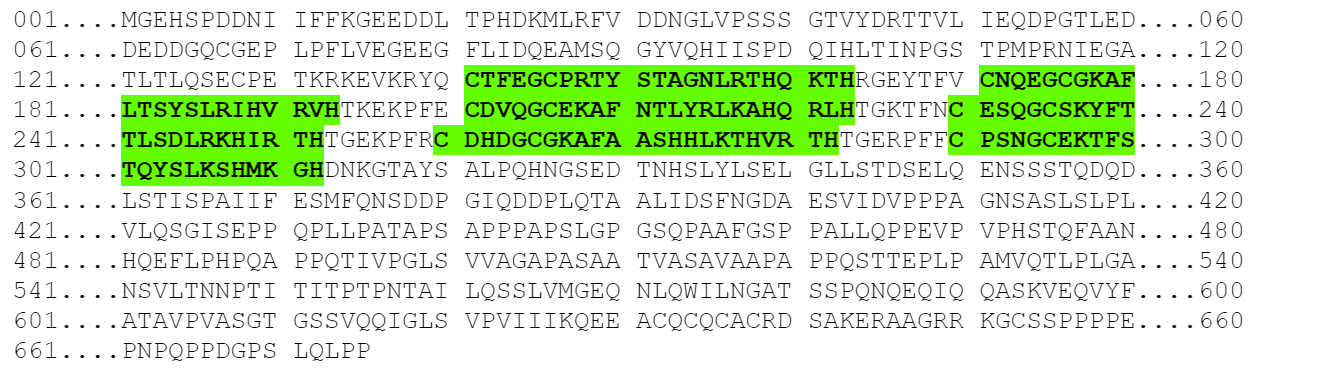
\includegraphics[width=.45\textwidth]{image/MusZF.png}}
	\subfigure[Fly MTF-1] {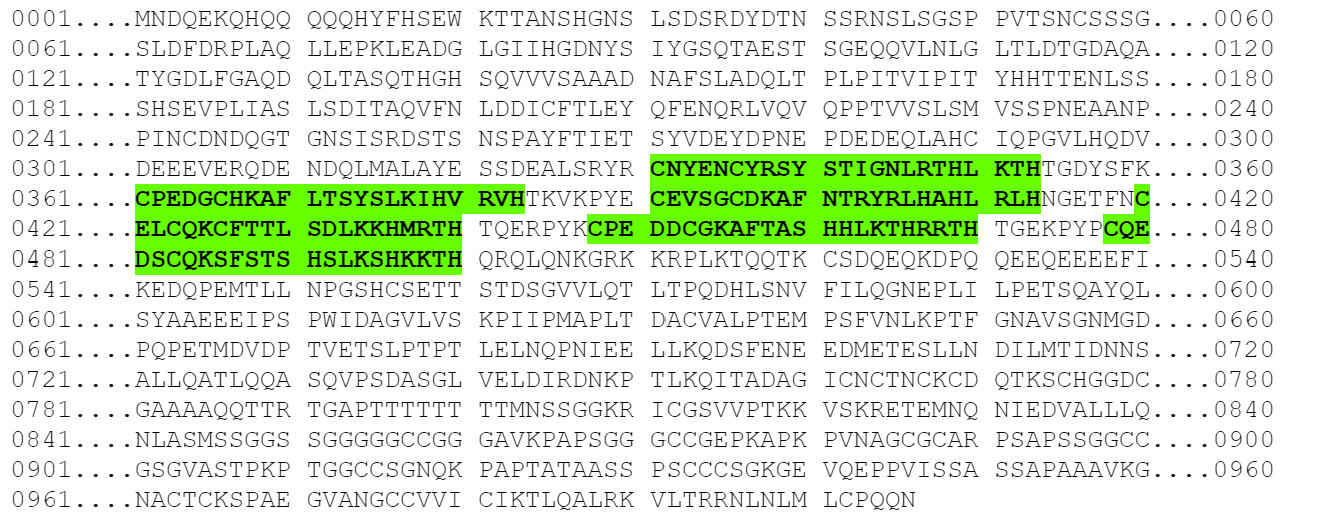
\includegraphics[width=.45\textwidth]{image/FlyZF.png}}
    \caption{Zinc finger prediction}
    \label{ZFP}
\end{figure}

Among the organisms we selected, most of them have the MTF-1 with 6 zinc finger domains, which is consistent with annotations in databases like uniprot.

\subsection{A consensus sequence named metal response elements can be found in a certain set of genes.}

Previous researches show that zinc finger can bind to a specific DNA sequence so that the protein can function on specific gene sequences. For transcription factors, zinc fingers can help them bind to the enhancers or upstream activation sequences so that they can recruit other transcription factors and RNA polymerase. Since the MTF-1 has zinc fingers, we wanted to know what sequence it can bind.

We used Interactive PWM Predictor, the DNA binding site predictor for Cys2His2 Zinc Finger Proteins\upcite{persikov2014novo}, to predict the binding sequence of MTF-1, and the results is shown below.

\begin{figure}[H]
    \centering
    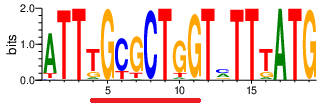
\includegraphics[width=0.9\textwidth]{image/seq_logo.png}
    \caption{Zinc finger binding sequence prediction}
    \label{ZCP}
\end{figure}

The detailed PWM can be found in Supplementary Material. From the figure above, we can find that the predicted consensus sequence is close to TGCRCNC reported in previous literature, indicating that this sequence is related to the function of MTF-1.

In other organisms, like \textit{Mus musculus} and \textit{Drosophila melanogaster}, the consensus sequence is highly similar.

\subsection{Expression of a certain set of genes with metal response elements may be regulated by MTF-1.}

We searched the human genome for the consensus sequence TGCRCNC, and 588381 hits are found. Among these hits, 126415 are close to an exon. We then compared the data to the annotation and gene ontology, and found several genes that can possibly be regulated by MTF-1 via the consensus sequence named metal response elements. These genes are listed below.

\begin{enumerate}
    \item MT/metallothionein
    \item HAMP/hepcidin
    \item PRNP/major prion protein
    \item DDAH1/N(G),N(G)-dimethylarginine dimethylaminohydrolase 1
\end{enumerate}

Then we did an analysis on the data series GSE76510\upcite{hardyman2016zinc} from GEO, which is a data set collected using Illumina HumanHT-12 V4.0 expression beadchip. In the experiment, a targeted siRNA was used to deplete MTF1 expression in the human intestinal cell line Caco-2, so that when the cell are treated with different zinc level, we can observe the difference in gene expression between the MTF-1 knockdown group and the control group. In this way, we can get more understanding of the MTF-1 regulated zinc-responsive genes expression.

The top differently expressed genes are listed below.

\begin{enumerate}
    \item HSPA6: heat shock protein family A (Hsp70) member 6
    \item MT1E:	metallothionein 1E
    \item MT1H:	metallothionein 1H
    \item RNA5S9:	RNA, 5S ribosomal 9
    \item MT1M:	metallothionein 1M
    \item SNORD3A:	small nucleolar RNA, C/D box 3A
    \item SNORD3D:	small nucleolar RNA, C/D box 3D
    \item MT1B:	metallothionein 1B
    \item MT1A:	metallothionein 1A
    \item SNORD3C:	small nucleolar RNA, C/D box 3C
    \item RN7SK:	RNA, 7SK small nuclear
    \item MT1F:	metallothionein 1F
    \item MT1G:	metallothionein 1G
    \item SERPINE2:	serpin family E member 2
    \item MT2A:	metallothionein 2A
    \item SLC30A1:	solute carrier family 30 member 1
    \item MT1X:	metallothionein 1X
    \item HSPA1A:	heat shock protein family A (Hsp70) member 1A
\end{enumerate}

Metallothioneins, as well as other genes, seem to be related to the change in MTF-1, which suggests that expression of a certain set of genes may be regulated by MTF-1. Some of them have metal response elements upstream several kbs of the gene.